\documentclass{beamer}
% \usepackage{animate}
\usepackage{multimedia}
\usepackage[english,russian]{babel}

\usepackage{pgfpages}
\setbeameroption{show notes on second screen}
%https://tug.ctan.org/macros/latex/contrib/beamer/doc/beameruserguide.pdf

\usepackage[T2A]{fontenc}
\usepackage[utf8]{inputenc}

\setbeamertemplate{caption}[numbered]

\usetheme{CambridgeUS}
\usecolortheme{dolphin}


\title[Физически-корректный рендеринг]{Физически-корректный рендеринг \\ Physically-Based Rendering}
\author[Быковских Д.А.]{Быковских Дмитрий Александрович}
\date{07.12.2024}

\begin{document}
	\begin{frame}
		\titlepage
	\end{frame}
	% \begin{frame}{Содержание}
	% \end{frame}
	%\section{Обзор}
	\begin{frame}{Введение}
		
		Физически-корректный рендеринг (Physically-Based Rendering, PBR)~---~метод рендеринга, основанный на физических принципах взаимодействия света с материалами. \\
		Цель PBR~---~создание более реалистичных и физически правильных изображений, учитывая разнообразные характеристики материалов и их взаимодействие со светом.

		Эти принципы позволяют PBR создавать более реалистичные материалы, которые лучше соответствуют поведению света в реальном мире.
		
		%В PBR широко используются такие модели, как Cook-Torrance для отражения и GGX для описания микрогеометрии поверхности.
	
		Популярные движки для 3D-графики, такие как Unreal Engine и Unity, включают поддержку PBR, что позволяет художникам и разработчикам создавать более реалистичные и красочные сцены.


		% Два подхода
		% В данной серии туториалов мы сосредоточимся на подходе PBR, первоначально разработанном в Disney и адаптированным для реал-тайм визуализации компанией Epic Games. Их подход, базирующийся на металл-диэлектрическом рабочем процессе (англ. metallic workflow, перевода лучше не нашел — прим. ред.), неплохо документирован, широко принят во многих популярных движках и выглядит потрясающе.

		

		\note{ \footnotesize
			Основные принципы PBR включают:
			\begin{itemize}
				\item 
				Сохранение энергии. Суммарная энергия света, падающего на поверхность, должна быть больше или равной суммарной энергии, излучаемой, отраженной и преломленной этой поверхностью.
				\item 
				Многолучевое преломление и отражение. Учет нескольких путей, которые может пройти свет через материал, включая преломление (прохождение света сквозь материал) и отражение.
				\item 
				Глобальное освещение. Интеграция различных источников света, включая прямое освещение от источников света и косвенное освещение от отраженного света.
				\item 
				Микрогеометрия поверхности. Учет микроструктуры поверхности материала, включая микрограни, которые влияют на отражение света.
				\item 
				Консистентность Френеля. Учет того, как интенсивность отражения меняется в зависимости от угла зрения и материала (свойство металличности).
			\end{itemize}			
		}

	\end{frame}

	\begin{frame}{Теория переноса света}{Закон сохранения энергии}
		
		Закон сохранения энергии~---~основной принцип, утверждающий, что в изолированной системе полная энергия остается постоянной. 
		
		Это означает, что энергия не может быть создана или уничтожена, она может только изменять свою форму.
		
		Этот закон особенно важен при рассмотрении взаимодействия света с различными поверхностями и средами. 

		Применительно к свету упрощенный закон сохранения энергии может быть выражен следующим образом ($\geqslant$ заменяется на $\approx $):
		
		\[ E_{\text{вх}} \geqslant E_{\text{отр}} + E_{\text{пр}} + E_{\text{погл}} 
		,\]
		где
		\(E_{\text{вх}}\)~---~энергия падающего света (входящая энергия);
		\(E_{\text{отр}}\)~---~энергия отраженного света;
		\(E_{\text{пр}}\)~---~энергия преломленного света (если свет проходит через среду с изменением показателя преломления);
		\(E_{\text{погл}}\)~---~энергия поглощенного света.
		
		\note{
			% При отражении света от зеркальной поверхности или при преломлении света при переходе из одной среды в другую (например, из воздуха в стекло) закон сохранения света остается соблюденным.
			\begin{figure}
				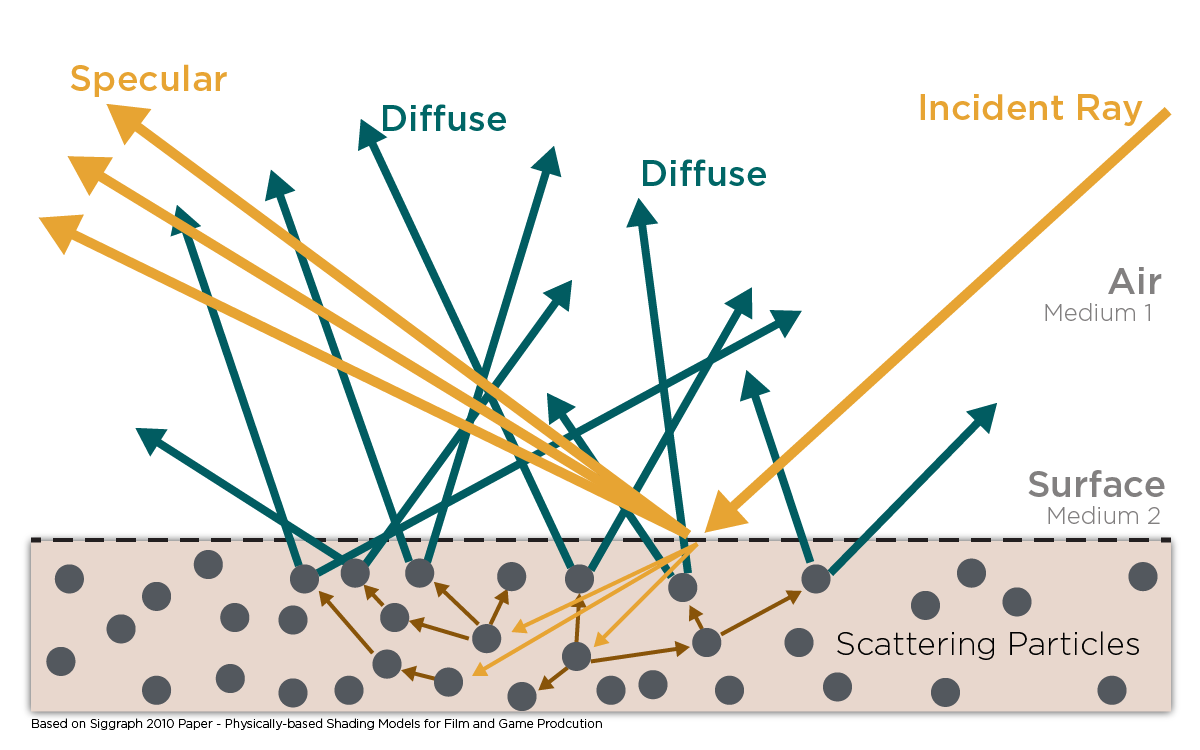
\includegraphics[width=0.85\textwidth]{images/theory_of_light_.png}
				\caption{Взаимодействие света с поверхностью}
			\end{figure}
		}


	\end{frame}



	\begin{frame}{Подповерхностное рассеивание}

		Подповерхностное рассеяние света происходит, когда свет поглощается и рассеивается внутри материала под его поверхностью. 
		
		Этот процесс часто встречается в различных средах, таких как вода, молекулярные газы, стекло, биологические ткани и другие.
		
    Рассеивание света внутри материала может зависеть от длины волны, что может создавать эффекты цветного рассеяния.

		Основные аспекты подповерхностного рассеяния:
		{\footnotesize
		\begin{itemize}
			\item 
			Рассеивание света внутри материала. Поглощенный свет может рассеиваться внутри материала, из-за чего часть его энергии может вернуться на поверхность.
			\item 
			Изменение направления света. Свет, попадающий в материал, может изменять свое направление из-за взаимодействия с молекулами или частицами внутри.
			\item 
			Эффекты мутности и мягких краев. Подповерхностное рассеяние может создавать эффекты мутности в материалах, а также способствовать формированию мягких краев и более плавных переходов между освещенными и теневыми областями.
		\end{itemize}
		}
		
		%Визуализация подповерхностного рассеяния часто требует сложных алгоритмов в компьютерной графике, таких как симуляция с использованием методов трассировки лучей или подходов, основанных на моделировании светового транспорта. Эти методы позволяют создавать более реалистичные и естественные изображения, учитывая сложные взаимодействия света с материалами.

		\note{
			% https://demiart.ru/forum/index.php?showtopic=146834
			\begin{figure}
				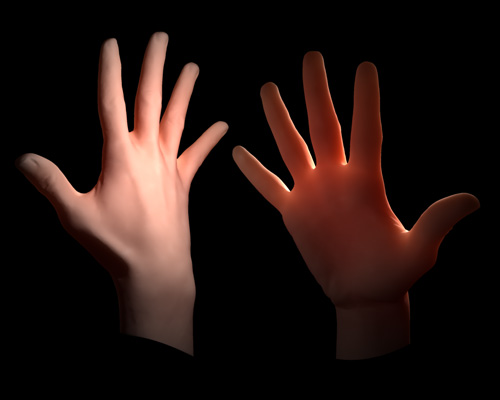
\includegraphics[width=0.6\textwidth]{images/hands.jpg}
				\caption{Подповерхностное рассеяние лучше всего заметно на тонкой геометрии, как кожа между пальцами}
			\end{figure}
		}
	\end{frame}

	\begin{frame}{Шероховатость поверхности}

		Шероховатость поверхности определяет степень неровности или нерегулярности поверхности. 
		
		Она описывает, насколько мелкие детали, бугры или выемки присутствуют на поверхности объекта.
		
		Она влияет на то, как свет взаимодействует с поверхностью и какие эффекты она создает. 



		\begin{figure}
			
\includegraphics[width=0.95\textwidth]{images/rough_and_smooth_surfaces.png}
			\caption{Сравнение поверхностей с разной степенью шероховатости}
		\end{figure}

		\note{

		Таким образом, шероховатость поверхности тесно связана с тем, как свет взаимодействует с объектом, и она играет важную роль в создании реалистичных изображений в компьютерной графике.

		}

	\end{frame}





	\begin{frame}{Медианный вектор}{halfway vector}
		
		Для расчета отраженной компоненты требуется выполнить довольно громоздкие вычисления. Существует модель Блинна-Фонга, представляющая собой модель Фонга с упрощенным расчетом зеркального отражения. Вычислим в каждой точке медианный вектор ${H}$ (halfway vector):
		\[
			H=\frac{L+V}{|L+V|}
			,
		\]
		который показывает ориентацию площадки, на которой будет максимальное отражение. 
		\note{
			\begin{figure} 
				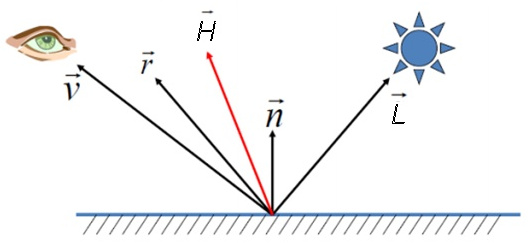
\includegraphics[width=0.95\textwidth]{images/halfway_vector.jpg}
				\caption{Пример расположения векторов}
			\end{figure}
			}
	\end{frame}


		\begin{frame}{Физически-корректный рендеринг}{Physically-Based Rendering}
	
		Физически-корректный рендеринг (Physically Based Rendering, PBR)~---~подход к генерации изображений, который стремится моделировать физические свойства света и материалов для достижения более реалистичных результатов.

		Излученность в направлении наблюдения при условии всех входящих световых потоков. 
		% \[
		% 	L(x, \theta_o, \phi_o) = 
		% 	\int_{\Omega} 
		% 	%\text{BRDF}
		% 	f_r(x, \theta_o, \phi_o, \theta_i, \phi_i) 
		% 	L(x, \theta_i, \phi_i) 
		% 	\cos \theta_i d \omega_i
		% \]
		\[
			L(x, \omega_o) 
			=
			\int_{\Omega_+} 
			f_r(x, \omega_o, \omega_i) 
			L(x, \omega_i) 
			(n \cdot \omega_i)
			d \omega_i
		\]
		где 
		$
			%\text{BRDF}
			f_r(x, \omega_o, \omega_i) 
			% =
			% \frac{d L(x, \theta_o, \phi_o)}{d E (x, \theta_i, \phi_i)}
		$~---~двулучевая функция отражательной способности (Bidirectional Reflectance Distribution Function, BRDF).
		

		\note{
		\begin{figure}
			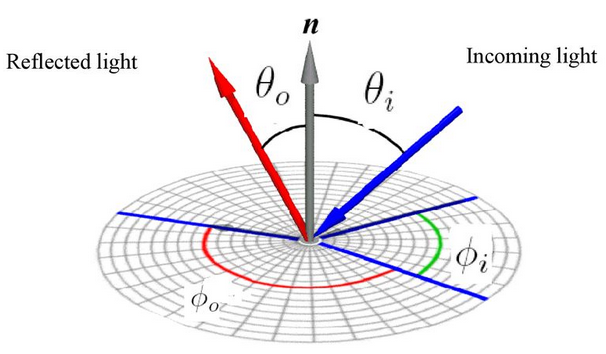
\includegraphics[width=0.8\textwidth]{images/brdf_2.png}
			\caption{Двулучевая функция отражательной способности}
		\end{figure}
		}
	\end{frame}

	\begin{frame}{Физически-корректный рендеринг}{Physically-Based Rendering}

		Существует несколько физически-корректных моделей BRDF для аппроксимации реакции поверхности на освещение. Самой популярной является модель BRDF Кука-Торренса 
		(Cook-Torrance), которая содержит диффузную и зеркальную составляющие:
		
		\[
			f_r =
			k_d f_{\text{lambert}}
			+
			k_s f_{\text{cook-torrance}} 	
		\]
		где 
		$k_d$~---~преломленная доля входящей световой энергии;
		$k_s$~---~отраженная доля входящей световой энергии.

		\[
			f_r =
			k_d \frac{c}{\pi} 
			+
			k_s \frac{DFG}{4 (\omega_o \cdot n) (\omega_i \cdot n)} 	
		,
			\]
		где 
		$c$~---~альбедо или цвет поверхности (диффузная текстура поверхности).

		
		
		
		\note{
			% $4 (\omega_o \cdot n) (\omega_i \cdot n)$

		% Уравнение отражения Кука-Торренса. \\

			% Первое слагаемое BRDF описывает диффузную часть уравнения, обозначенную здесь как $f_{\text{lambert}}$. Это есть Ламбертово рассеяние.
			% \\
			% Примечание.
			% Деление на $\pi$ нужно, чтобы нормировать рассеянный свет, поскольку ранее обозначенный интеграл, содержащий BRDF, умножается на $\pi$.
			
			% \begin{figure} 
			% 	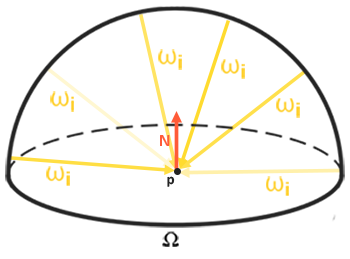
\includegraphics[width=0.65\textwidth]{images/w_i_and_omega.png}
			% 	\caption{Иллюстрация усредненной суммы энергетической яркости внутри полусферы}
			% \end{figure}
		}
	\end{frame}

	\begin{frame}{Физически-корректный рендеринг}{Physically-Based Rendering}
		% https://dspace.susu.ru/xmlui/bitstream/handle/0001.74/30326/73_77.pdf?sequence=1&isAllowed=y


		Существует несколько физически-корректных BRDF для аппроксимации реакции поверхности на освещение. Тем не менее, почти все графические конвейеры реального времени используют BRDF, известную как BRDF Кука-Торренса (Cook-Torrance).

		\[
			L (x, \omega_0) =
			% M (x, w_o) +
			\int_{\Omega_+} \bigg( 
			k_d \frac{c}{\pi} 
			+
			k_s \frac{DFG}{4 (\omega_0 \cdot n) (\omega_i \cdot n)} 
			\bigg)
			L (x,\omega_i) (n \cdot \omega_i)
			d \omega_i
		\]

		\note {
			\footnotesize
			Основные принципы физически-корректного рендеринга включают в себя:

			\begin{itemize}
				\item 
				Моделирование света.
				Учет различных источников света, их цветовых температур, направления и интенсивности.
				Учет закона сохранения энергии в процессе отражения и преломления света.
				\item 
				Моделирование материалов.
				Физически-корректные модели отражения, преломления и поглощения света в зависимости от типа материала.
				\item 
				Моделирование теней и окружающей среды.
				Учет влияния теней от различных объектов и источников света.
				Моделирование окружающей среды для более точного воссоздания условий освещения.
				\item 
				Многоканальные текстуры.
				Использование текстур с несколькими каналами для более точного представления различных характеристик материалов, таких как шероховатость, металлические свойства и др.
				\item 
				Моделирование камеры.
				Учет характеристик камеры, таких как диафрагма и выдержка, для более реалистичного эффекта глубины резкости и затемнения по краям кадра.
			\end{itemize}
		}

	\end{frame}

	\begin{frame}{Диффузное рассеивание}

		Первое слагаемое BRDF описывает диффузную часть уравнения, обозначенную здесь как $f_{\text{lambert}}$. Это есть Ламбертово рассеяние.
		\[
				L_o(x,\omega_o) = k_d \frac{c}{\pi}
				\int_{\Omega}
				L_i(x, \omega_i) (n \cdot \omega_i) d \omega_i
			,
			\]
			где 
			$\omega_i$~---~входящий вектор направления рассчитывается случайным образом с некоторым законом распределения.

			\footnotesize
			Примечание. \\
			Деление на $\pi$ нужно, чтобы нормировать рассеянный свет, поскольку ранее обозначенный интеграл, содержащий BRDF, умножается на $\pi$.

	\end{frame}

	\begin{frame}{Зеркальное рассеивание}



		Второе слагаемое $k_s f_{\text{cook-torrance}}$ выглядит немного сложнее и описывает зеркальную часть уравнения.
		
		\[
			L_o(x,\omega_o) = 
			k_s 
			\int_{\Omega} 
			\frac{D F G}{4 (\omega_o \cdot n) (\omega_i \cdot n)} 
			L_i(x,\omega_i) (n \cdot \omega_i)
			d \omega_i
		,
		\]
			где 
			$\omega_i$~---~входящий вектор направления рассчитывается случайным образом с некоторым законом распределения.

			\footnotesize
			Примечание. \\
			Это слагаемое состоит из трех функций и коэффициента нормирования в знаменателе. Каждая из букв $D$, $F$ и $G$ представляет собой определенный тип функции, которая аппроксимирует определенную часть отражающих свойств поверхности.

			\note{			
			
				\begin{enumerate}
					\item 
					Функция нормального распределения (Normal Distribution Function, NDF) аппроксимирует количество микрограней поверхности, ориентированных по медианному вектору, основываясь на шероховатости поверхности; это основная функция, аппроксимирующая микрограни.
					\item
					Уравнение Френеля (Fresnel Equation) описывает коэффициент поверхностного отражения при разных углах.
					\item
					Функция геометрии (Geometry Function) описывает свойство самозатенения микрограней. Когда поверхность довольно шероховатая, одни микрограни поверхности могут перекрывать другие, тем самым уменьшая количество света, отражаемого поверхностью.
				\end{enumerate}

							
				Каждая из этих функций имеет различные реализации, направленные на приближенное описание заданной физической модели.
				

			}

	\end{frame}

% 	\begin{frame}{Зеркальное рассеивание}
% 		Trowbridge-Reitz GGX для D (распределение нормалей):
% 		Trowbridge-Reitz GGX (англ. Generalized Trowbridge-Reitz Geometric optics reflectance model) представляет собой распределение вероятности для направлений микроповерхностей поверхности. Оно используется в функции распределения вероятности (D), которая описывает, как нормали на поверхности распределены.

% Приближение Френеля-Шлика для F (коэффициент Френеля):
% 		Приближение Френеля-Шлика (англ. Schlick's approximation) часто используется для приближенного вычисления коэффициента Френеля, который описывает, как свет отражается от поверхности в зависимости от угла падения света и угла обзора. Это приближение часто бывает удобным для вычислений в реальном времени.

% Smith's Schlick-GGX для G (Функция геометрии):
% 		Smith's Schlick-GGX (англ. Smith's Schlick-GGX geometric shadowing function) используется для вычисления геометрического коэффициента (G), который учитывает тень, бросаемую микроповерхностями на поверхности. Этот коэффициент влияет на то, как свет проходит через микроструктуру поверхности и влияет на конечный результат отражения.

% 		\note{
% 			Таким образом, комбинация этих компонентов - D, F и G - вместе с учетом направления Астичного моделирования отражения света и теней на 3D-объектах.
% 		}

% 	\end{frame}

	\begin{frame}{Функция нормального распределения (D)}{}
		В физически-корректном рендеринге (PBR), модель микрограней используется для описания микроструктуры поверхности материала и её влияния на отражение света. 
		Одной из широко используемых моделей микрограней является GGX (англ. Generalized Trowbridge-Reitz Geometric optics reflectance model).
		
		Функция нормального распределения D статистически аппроксимирует относительную площадь поверхности микрограней, точно ориентированных по медианному вектору $h$.
		
		\[ 
			D(\mathbf{n, h, \alpha}) = \dfrac{\alpha^2}{\pi ((\mathbf{h} \cdot \mathbf{n})^2 (\alpha^2 - 1) + 1)^2} 
			,
		\]
		где
		\(D\) - функция распределения вероятности микрограней;
		\(\mathbf{n}\) - нормаль к поверхности;
		\(\mathbf{h}\) - медианный вектор;
		\(\alpha\) - параметр шероховатости (roughness) поверхности.
		
		\note{

		% https://tryingtobeananimator.wordpress.com/2018/11/25/technical-ggx-vs-beckham-why-and-whats-the-difference/

			\begin{figure}
				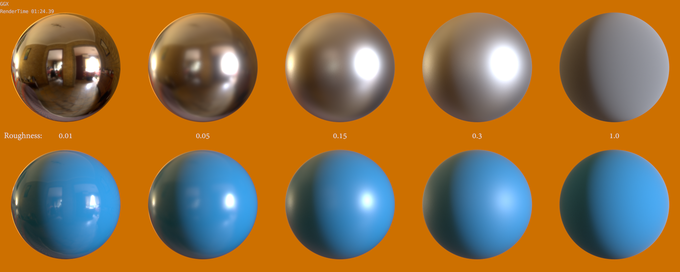
\includegraphics[width=0.9\textwidth]{images/gloss_ggx__small.png}
				\caption{Функция нормального распределения GGX при различных значениях шероховатости}
			\end{figure}

			\footnotesize
		% Модель GGX основана на теории микрогеометрии поверхности и учитывает распределение микрограней (микрограней) на поверхности материала. Эта модель описывает вероятность того, что свет будет отражаться под определенным углом от микрограни. 
		
		% 	Это распределение предоставляет более реалистичное описание, как свет взаимодействует с микроповерхностями на поверхности материала, и позволяет более точно моделировать отражение света в различных условиях.
			
			%Применение модели GGX обычно включает расчет отраженной интенсивности света (specular reflection) в уравнении освещения, учитывая микрогеометрию и другие параметры материала. Это 
			Примечание:
			способствует созданию более реалистичных изображений, особенно в отношении материалов с разной степенью шероховатости.
		}
		
	\end{frame}

	\begin{frame}{Уравнение Френеля-Шлика (F)}{Schlick's approximation of the Fresnel equation}
		

		Уравнение Френеля-Шлика (упрощенное уравнение Френеля) выглядит следующим образом:
		
		\[ F(\theta) = F_0 + (1 - F_0)(1 - \cos \theta)^5 ,\]
		где
		\( F(\theta) \)~---~коэффициент отражения света при угле падения \( \theta \);
		\( F_0 \)~---~коэффициент отражения при нормальном угле падения (\( \theta = 0 \));
		\( \cos \theta \)~---~косинус угла падения света.
		
		\footnotesize
		Примечание.

		Показатель преломления $F_0$ или IOR (indices of refraction) вычисляется с использованием формулы:
		
		\[ F_0 = \left(\frac{n_1 - n_2}{n_1 + n_2}\right)^2 ,\]
		где
		\( n_1 \)~---~показатель преломления первой среды (например, воздуха);
		\( n_2 \)~---~показатель преломления второй среды (например, материала).
		
		% Уравнение Френеля-Шлика обычно используется для моделирования отражения на поверхностях с различными свойствами, такими как стекло, пластик или вода. Оно позволяет аппроксимировать изменение отражательности в зависимости от угла падения света без сложных вычислений, что особенно полезно в реальном времени или при ограниченных вычислительных ресурсах.
		
		\note{
			% Уравнение Френеля-Шлика (Schlick's approximation of the Fresnel equation) представляет собой упрощенную формулу для вычисления коэффициента отражения света от поверхности при падении света под углом. Эта аппроксимация была предложена Джоном Шликом (John Schlick) и широко используется в компьютерной графике из-за своей простоты и эффективности.
			
			% https://vivareit.ru/samye-chistye-ozera-rossii-kristalnaya-semerka/
			% https://shanesimmsart.wordpress.com/2022/03/29/fresnel-reflection/
			\begin{figure}
				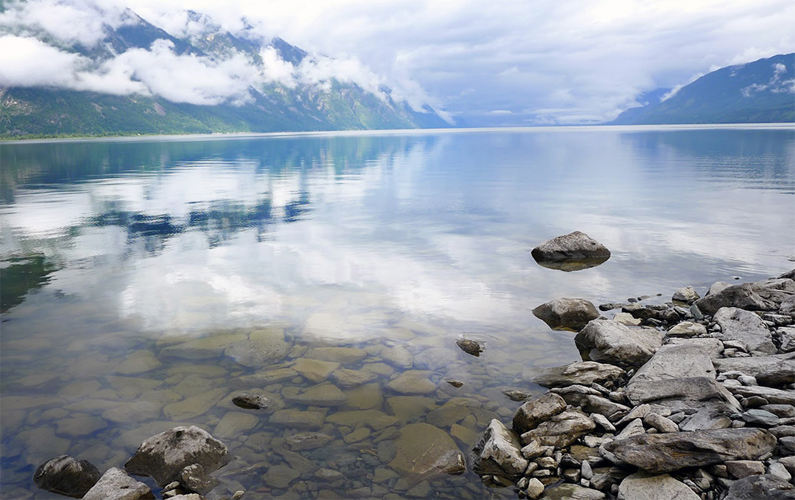
\includegraphics[width=0.85\textwidth]{images/telec_lake.jpg}
				\caption{Телецкое озеро, Республика Алтай}
			\end{figure}
		
		}
			\end{frame}

	\begin{frame}{Функция геометрии (G)}{}
		Функция геометрии статистически аппроксимирует относительную площадь поверхности, где ее микроскопические неровности перекрывают друг друга, что не дает проникать световым лучам.

		Функция геометрии представляет собой комбинацию приближения GGX и Шлика-Бекмана (Schlick-Beckmann), и известна как Schlick-GGX:

		\[
			G_{\text{SchlickGGX}}(n,v,k)=\frac{n\cdot v}{(n\cdot v)(1-k)+k}
			\]



		Чтобы эффективно аппроксимировать геометрию, нам необходимо учитывать как направление обзора (перекрытие геометрии), так и вектор направления света (самозатенение геометрии). Мы можем учитывать оба случая с помощью метода Смита:

		\[
			G(n,v,l,k)=G_{sub}(n,v,k)G_{sub}(n,l,k)
			\]

		
		\note{

			\begin{figure}
				
\includegraphics[width=0.9\textwidth]{images/geometry_function.png}
				\caption{Пример перекрытия и самозатенения геометрии}
			\end{figure}

			\footnotesize
			Здесь $k$ является переобозначением $\alpha$ в зависимости от того, используем ли мы функцию геометрии для прямого освещения или освещения IBL:
			$k_{direct}=\frac{(\alpha+1)^2}{8}$;
			$k_{IBL}=\frac{\alpha^2}{2}$.
		}
		
	\end{frame}



	\begin{frame}{Текстурирование и материалы}
		% https://www.youtube.com/watch?v=yQig4ax1S8A
		% https://habr.com/ru/articles/458696/

{	\footnotesize	
	В контексте PBR для определения характеристик материала используется два подхода, различающиеся следующими наборами параметров:

		\begin{enumerate}
			\item 
			Color-Metal-Roughness:
			
			Metallic (Металличность). %Определяет, является ли материал металлическим или нет. 
			Значение 0 обозначает неметаллический материал, а значение 1 - металлический. 
			%Для нескольких материалов между этими значениями можно использовать интерполяцию.
			
			Roughness (Шероховатость). %Определяет, насколько материал шершавый или гладкий. 
			%Значение 0 соответствует абсолютно гладкой поверхности, а 1 - максимальной шероховатости. 
			Чем выше значение, тем более рассеянным и размытым будет отраженный свет.
			
			\item
			Diffuse-Specular-Glossiness:
			
			Specular (Зеркальность). %Параметр, определяющий степень отражения света на гладкой поверхности. 
			Высокое значение соответствует более зеркальному отражению.
			
			Glossiness (Глянцевитость). %Альтернатива шероховатости в Metallic Roughness. 
			Глянцевитость определяет, насколько материал гладкий. 
			Значение 0 соответствует абсолютно гладкой поверхности, а 1~---~максимальной шероховатости.

	\end{enumerate}
		
		
Оба формата широко применяются в PBR-системах, и выбор между ними зависит от конкретных требований и удобства в работе с конкретным движком или программой для 3D-графики.

В целом, выбор между этими форматами зависит от конкретных требований проекта, предпочтений художников и уровня поддержки в используемом движке.
}
\note{
	% https://www.youtube.com/watch?v=yQig4ax1S8A
	\begin{figure}
		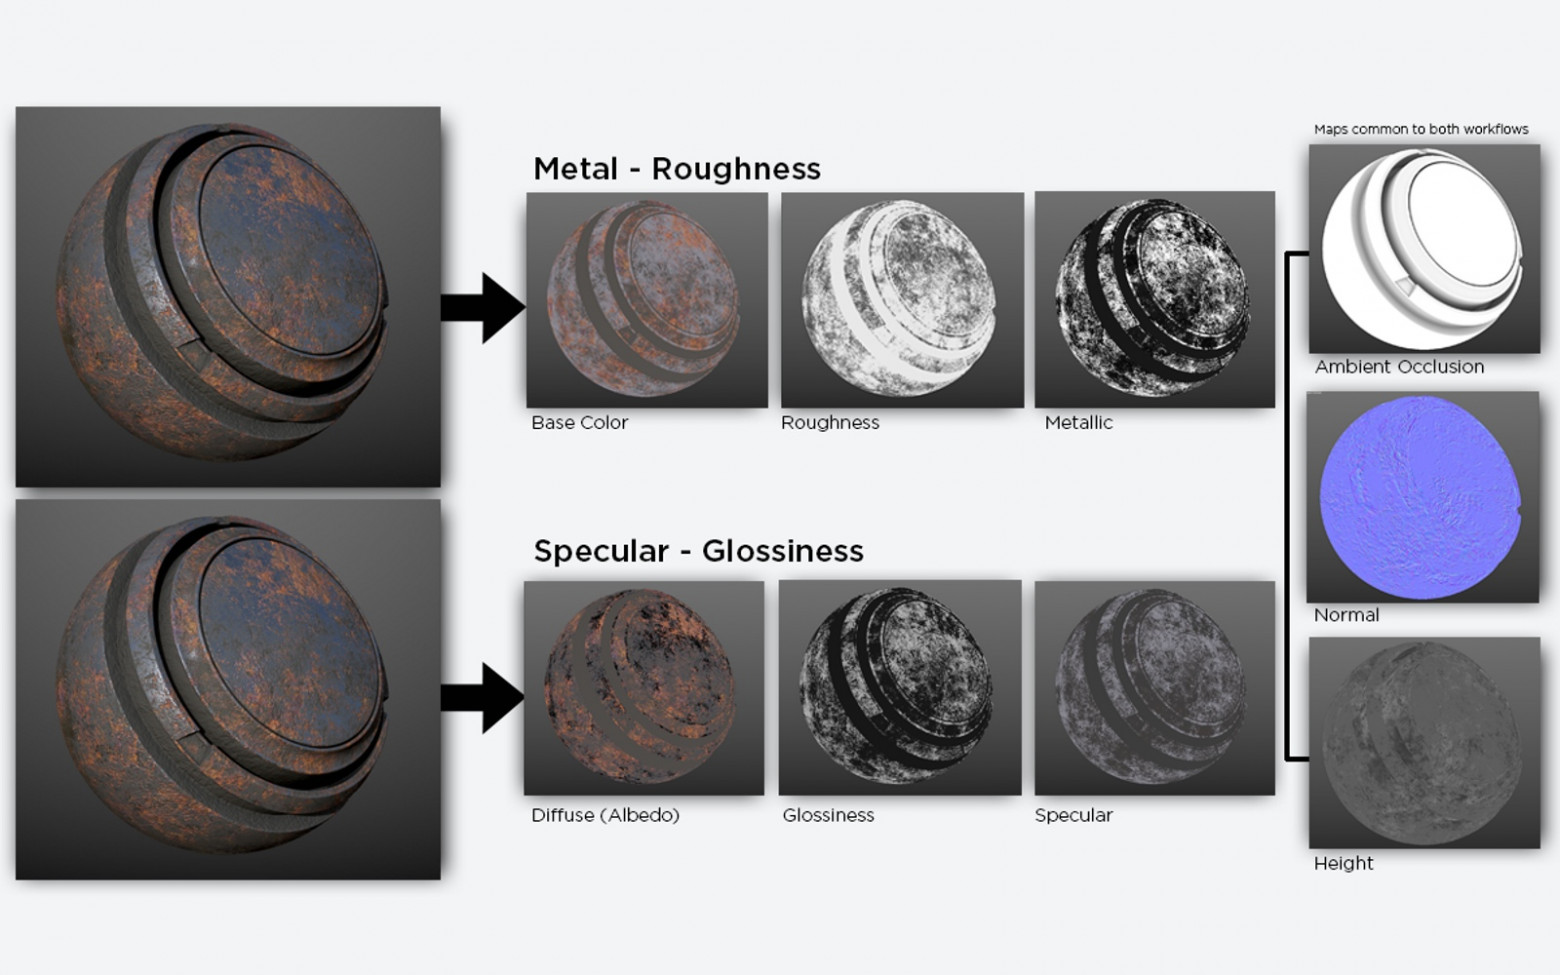
\includegraphics[width=0.9\textwidth]{images/MR_vs_SG.jpg}
		\caption{Сравнение Color-Metal-Roughness и Diffuse-Specular-Glossiness подходов}
	\end{figure}
}

	\end{frame}

	\begin{frame}{Создание материалов для PBR}
		
		% Физически-корректный рендеринг (PBR) стремится моделировать физические свойства материалов более точно.
		
		{
			\footnotesize
		Виды материалов

		\begin{enumerate}
			\item 
			Albedo (цвет или базовый цвет без учета теней и отражений).
			\item 
			Карта нормалей (Normal Map).
					Используется для добавления деталей к поверхности, не увеличивая сложности ее геометрию. 
			\item 
			Металличность (Metallic).
			\item 
			Шероховатость (Roughness).
			\item 
			Карта подсветки (Ambient Occlusion Map).
					Используется для задания затененных областей.
			\item 
					Карта окружающей среды (Environment Map).
							Используется или текстура, отображающая окружающий мир, или использование динамической карты окружения.
			\item
			Карта высот (Height Map).
					Используется для создания эффекта рельефа (высоты) или выпуклости на поверхности материала.
			\item
				Карта микроповерхностей (Microfacet Map).
				Обычно используется вместе с GGX-моделью для распределения микроповерхностей.
			\item
			Функции отражения и преломления (Fresnel).
			    Определяют, как свет взаимодействует с материалом при отражении и преломлении, могут использоваться в модели Френеля в уравнении отражения.
		\end{enumerate}
		
		% Каждый из этих элементов может быть регулируемым параметром или текстурой. %, что позволяет создавать более сложные и реалистичные материалы. %Различные программы и движки для 3D-графики могут предоставлять инструменты для настройки этих параметров и создания PBR-материалов.
		}
		
	\note{
			\begin{figure}
				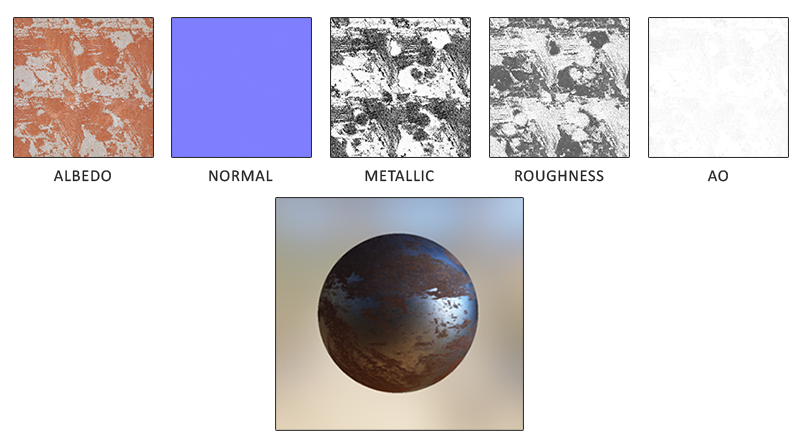
\includegraphics[width=0.9\textwidth]{images/materials.png}
				\caption{Примеры текстур}
			\end{figure}
		}
	\end{frame}

	\begin{frame}{Заключение}
		Литература
		\begin{enumerate}
			% \item \href{https://tug.ctan.org/macros/latex/contrib/beamer/doc/beameruserguide.pdf}{}
			% \item \href{https://demiart.ru/forum/index.php?showtopic=146834}{}
			\item \href{https://dspace.susu.ru/xmlui/bitstream/handle/0001.74/30326/73_77.pdf?sequence=1&isAllowed=y}{Чистяков А.В. Особенности алгоритмов физически корректного рендеринга для интерактивной архитектурной визуализации}
			\item \href{https://tryingtobeananimator.wordpress.com/2018/11/25/technical-ggx-vs-beckham-why-and-whats-the-difference/}{Technical – GGX vs Beckham}
			\item \href{https://vivareit.ru/samye-chistye-ozera-rossii-kristalnaya-semerka/}{Самые чистые озера России}
			\item \href{https://shanesimmsart.wordpress.com/2022/03/29/fresnel-reflection/}{Fresnel Reflection and Fresnel Reflection Modes Explained}
			\item \href{https://www.youtube.com/watch?v=yQig4ax1S8A}{PBR: Физически корректный рендеринг — сравнение Metallic Roughness и Specular Glossiness}
			\item \href{https://habr.com/ru/articles/458696/}{Кузнецов Д. Текстурирование. Часть 3. PBR и материалы}
		\end{enumerate}

	\end{frame}
	
\end{document}
